\documentclass[a0paper,portrait]{baposter}
\usepackage{wrapfig}
\usepackage{lmodern}
\usepackage[utf8]{inputenc} %unicode support
\usepackage[T1]{fontenc}
\selectcolormodel{cmyk}
\graphicspath{{figures/}} % Directory in which figures are stored
\usepackage{hyperref}
\newcommand{\compresslist}{\setlength{\itemsep}{0pt}\setlength{\parskip}{1pt}\setlength{\parsep}{0pt}}
\newenvironment{boenumerate}{\begin{enumerate}\renewcommand\labelenumi{\textbf\theenumi.}}{\end{enumerate}}

\begin{document}
	\definecolor{darkgreen}{cmyk}{0.8,0,0.8,0.45}
	\definecolor{lightgreen}{cmyk}{0.8,0,0.8,0.25}
	\begin{poster}
		{
			grid=false,
			headerborder=open, % Adds a border around the header of content boxes
			colspacing=1em, % Column spacing
			bgColorOne=white, % Background color for the gradient on the left side of the poster
			bgColorTwo=white, % Background color for the gradient on the right side of the poster
			borderColor=darkgreen, % Border color
			headerColorOne=lightgreen, % Background color for the header in the content boxes (left side)
			headerColorTwo=lightgreen, % Background color for the header in the content boxes (right side)
			headerFontColor=white, % Text color for the header text in the content boxes
			boxColorOne=white, % Background color of the content boxes
			textborder=rounded, %rectangle, % Format of the border around content boxes, can be: none, bars, coils, triangles, rectangle, rounded, roundedsmall, roundedright or faded
			eyecatcher=false, % Set to false for ignoring the left logo in the title and move the title left
			headerheight=0.11\textheight, % Height of the header
			headershape=rounded, % Specify the rounded corner in the content box headers, can be: rectangle, small-rounded, roundedright, roundedleft or rounded
			headershade=plain,
			headerfont=\Large\textsf, % Large, bold and sans serif font in the headers of content boxes
			%textfont={\setlength{\parindent}{1.5em}}, % Uncomment for paragraph indentation
			linewidth=2pt % Width of the border lines around content boxes
		}
		{}
		{
			{\small Projet de Fin d'Études 2022-2023}
			\sf\vspace{0.3em}\\
			\\\textsf
			{Navigation et contrôle multi-robots pour l'inspection acoustique de structures métallique}
		}
		{
			\sf\vspace{0.5em}\\
			Brandon ALVES
			\vspace{0.1em}\\
			\small{
				Département Informatique, INSA Lyon - CITI Lab. INSA - INRIA
				\vspace{0.2em}\\
				bdasilvaal@insa-lyon.fr
				\vspace{0.2em}\\
			}
		}
		{
			\hspace{0.5cm}
			
\includegraphics[height=1cm]{graphics/insa.jpg}
			\hspace{0.5cm}
			
\includegraphics[height=1cm]{graphics/citi.png}
		}
		\headerbox{1. Introduction}{name=introduction,column=0,row=0,span=2}{
			L'inspection acoustique des structures métalliques est une tâche importante dans divers domaines tels que l'industrie, la construction et la maintenance.
			Elle vise à détecter les défauts et les anomalies, ce qui peut être crucial pour garantir la sécurité et la durabilité des structures.
			Cependant, l'inspection acoustique des structures métalliques peut être une tâche complexe et exigeante, en particulier dans les cas où les structures sont vastes ou difficilement accessibles.
			Les méthodes traditionnelles d'inspection manuelle sont souvent limitées en termes d'efficacité, de précision et de couverture.
			Dans ce projet de fin d'études, nous proposons une approche basée sur la navigation et le contrôle multi-robots pour améliorer l'inspection acoustique des structures métalliques.
			L'idée est d'utiliser un groupe de robots autonomes équipés de capteurs acoustiques pour explorer et inspecter efficacement la structure.
		}
		\headerbox{2. Problématique}{name=model,column=2,row=0,span=1}{
			L'objectif principal de ce projet est de développer des algorithmes de navigation et de contrôle multi-robots, permettant une exploration coordonnée et une collecte de données acoustiques précises sur la structure métallique.
			Nous cherchons à :
			\begin{itemize}\compresslist
				\item Obtenir une couverture complète de la structure.
				\item Maximiser la précision de la cartographie des défauts sur la structure.
				\item Minimiser le temps nécessaire pour effectuer une inspection complète.
			\end{itemize}
			En abordant ces problématiques, notre projet de fin d'études vise à proposer une solution basée sur la navigation et le contrôle multi-robots pour améliorer l'inspection acoustique des structures métalliques.
		}
		\headerbox{3. Éléments techniques}{name=item,column=2,below=model,span=1}{
			Ces stratégies sont basées sur l'utilisation de robots de type "crawlers" équipés de capteurs tels qu'un capteur IMU, un capteur UGW pour l'émission et la réception d'ondes accoustiques et un capteur LIDAR. Les robots sont capables de se synchroniser pour se déplacer simultanément ou de manière alternée.

			\begin{center}
				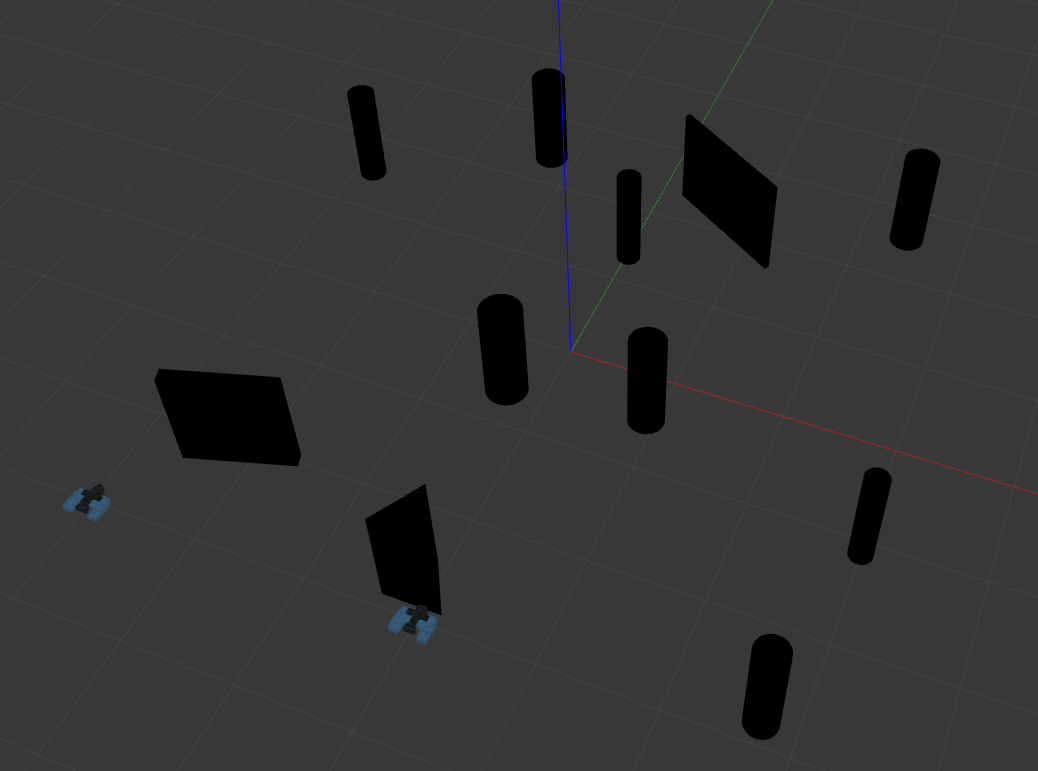
\includegraphics[width=\linewidth]{graphics/exemple_model.png}
			\end{center}

			Nous avons utilisé Gazebo pour simuler l'environnement et les robots, et ROS pour la communication entre les robots et le contrôle de la simulation.
		}
		\headerbox{4. Proposition de solution}{name=prop,span=2,column=0,below=introduction}{
			Nous proposons trois stratégies de navigation multi-robots pour l'inspection acoustique de structures métalliques, dans le but d'optimiser l'acquisition de données permettant de réaliser la tomographie des surfaces métalliques.
			Les trois stratégies sont les suivantes :
			\begin{boenumerate}\compresslist
				\item Stratégie de navigation \textit{peinture au rouleau} :
				Cette stratégie consiste en une exploration grossière de la surface à inspecter, où les robots se déplacent en ligne droite sur des trajectoires parallèles.
				Cette approche vise à obtenir rapidement une couverture globale de la surface à inspecter.
				Cette stratégie permet de quadriller la surface à inspecter et d'approcher les enveloppes convexes des zones de corrosion sous forme de rectangles.
				\item Stratégie de navigation \textit{ski nordique} :
				Cette stratégie est similaire à la stratégie \textit{peinture au rouleau}, mais les robots se déplacent de manière séquentielle plutôt que simultanée.
				Les robots se déplacent en ligne droite sur des trajectoires parallèles, avec des points d'arrêt différents pour chaque robot.
				Cette stratégie vise à augmenter la diversité d'orientation des rayons des signaux émis et reçu, ce qui permet d'approcher plus précisément les enveloppes convexes des zones de corrosion.
				\item Stratégie de navigation \textit{investigation polygonale} :
				Cette stratégie propose une approche plus précise pour l'inspection des zones potentielles de corrosion.
				Elle consiste en une exploration de la surface métallique en suivant des trajectoires polygonales.
				Les robots se déplacent en formant des polygones qui couvrent les zones à inspecter, permettant ainsi une meilleure approximation des enveloppes convexes des zones de corrosion.
			\end{boenumerate}
			% \begin{boenumerate}\compresslist
			% 	\item Stratégie de navigation \textit{peinture au rouleau} :
			% 	\item Stratégie de navigation \textit{ski nordique} :
			% 	\item Stratégie de navigation \textit{investigation polygonale} :
			% \end{boenumerate}
			% \begin{center}
			% 	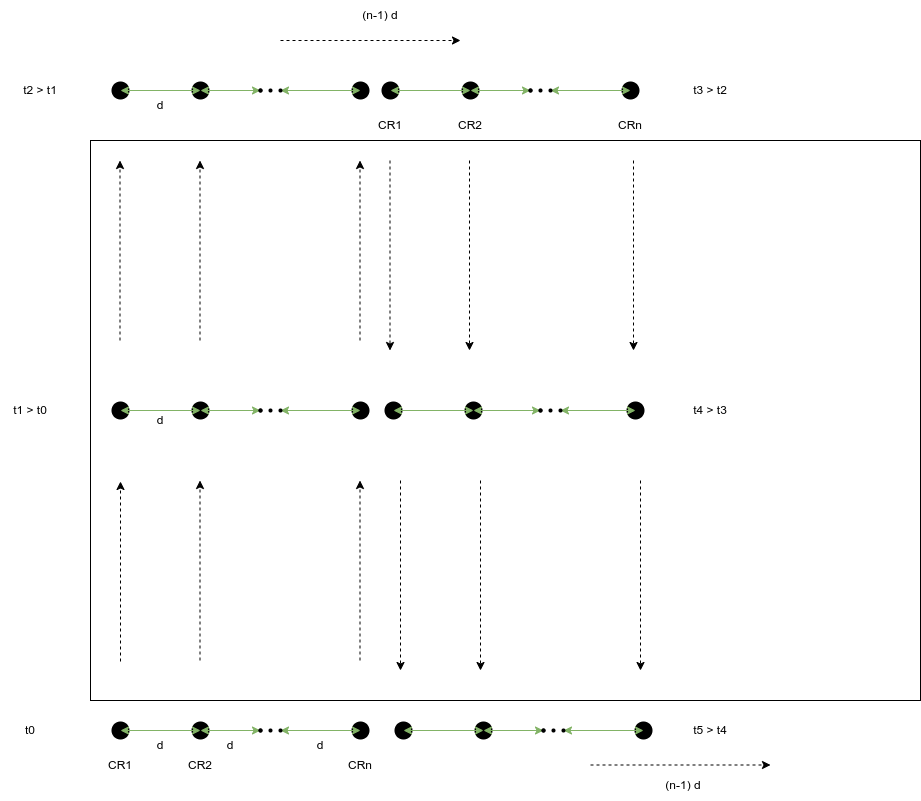
\includegraphics[width=0.45\linewidth]{graphics/peinture_au_rouleau.png}
			% 	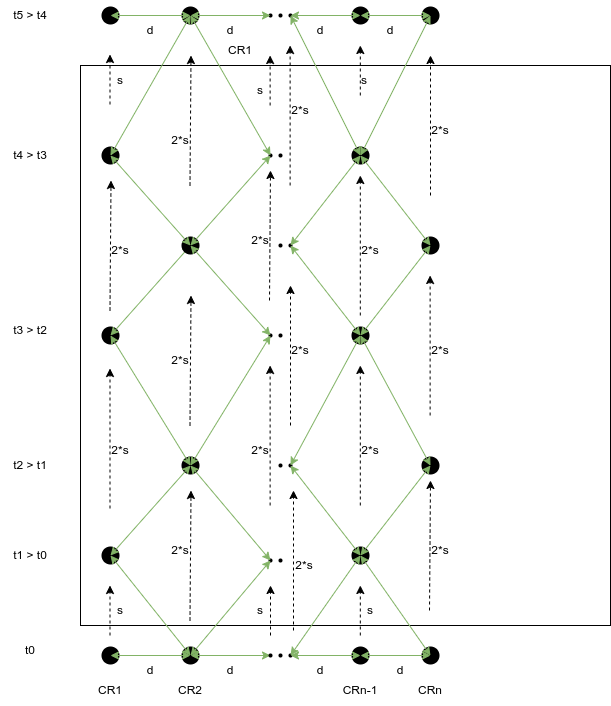
\includegraphics[width=0.45\linewidth]{graphics/ski_nordique_1.png}
			% 	% 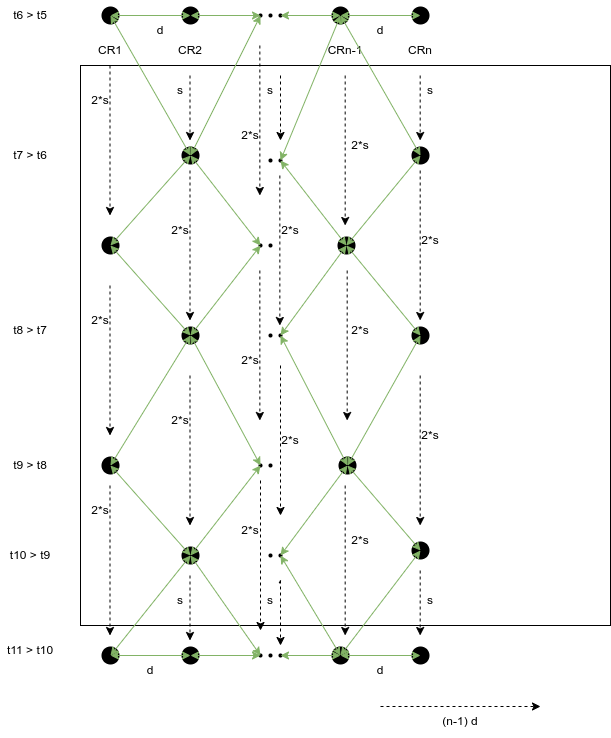
\includegraphics[width=0.3\linewidth]{graphics/ski_nordique_2.png}
			% 	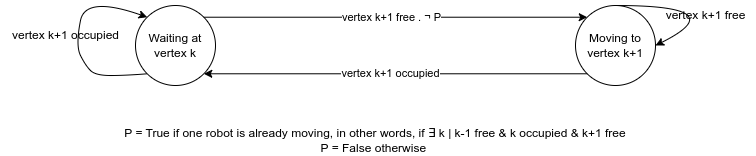
\includegraphics[width=0.9\linewidth]{graphics/automat_poly.png}
			% \end{center}
			Une grille d'occupation est utilisée pour modéliser l'environnement et obtenir en temps réel l'état de la surface métallique pendant l'inspection.
		}
		\headerbox{5. Évaluation de la proposition}{name=eval,span=2,column=0,below=prop,above=bottom}{
			Nous avons modélisé plusieurs cartes de tests qui modélisent une surface plane comportant différentes formes géométriques représentant les zones de corrosion à détecter et à localiser.
			La densité de corrosion des cartes varie.
			Nous avons évalué les performances des trois stratégies en termes de concordance avec la réalité et de temps d'inspection.
			Pour la stratégie "peinture au rouleau" et la stratégie "ski nordique", nous avons fait varier la distance entre les robots pour évaluer son impact sur les performances.
			Pour la stratégie "ski nordique", nous avons également fait varier le pas entre les robots.
			Pour la stratégie "investigation polygonale", nous avons fait varier le nombre de côtés des polygones utilisés.
			Lors de nos expérimentations, nous avons enregistré les valeurs du coefficient kappa de Cohen et du temps d'inspection pour chaque combinaison de paramètres.

			\begin{center}
				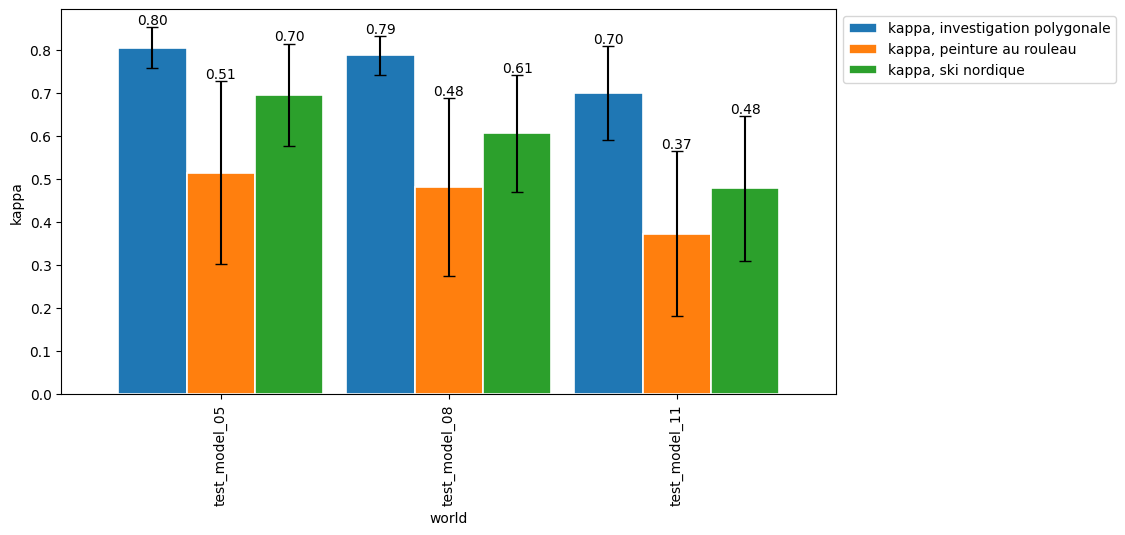
\includegraphics[width=0.49\linewidth]{graphics/investigation_polygonale-peinture_au_rouleau_ski_nordique-kappa_for_each_world_vs_investigation_polygonale-kappa_for_each_world.png}
				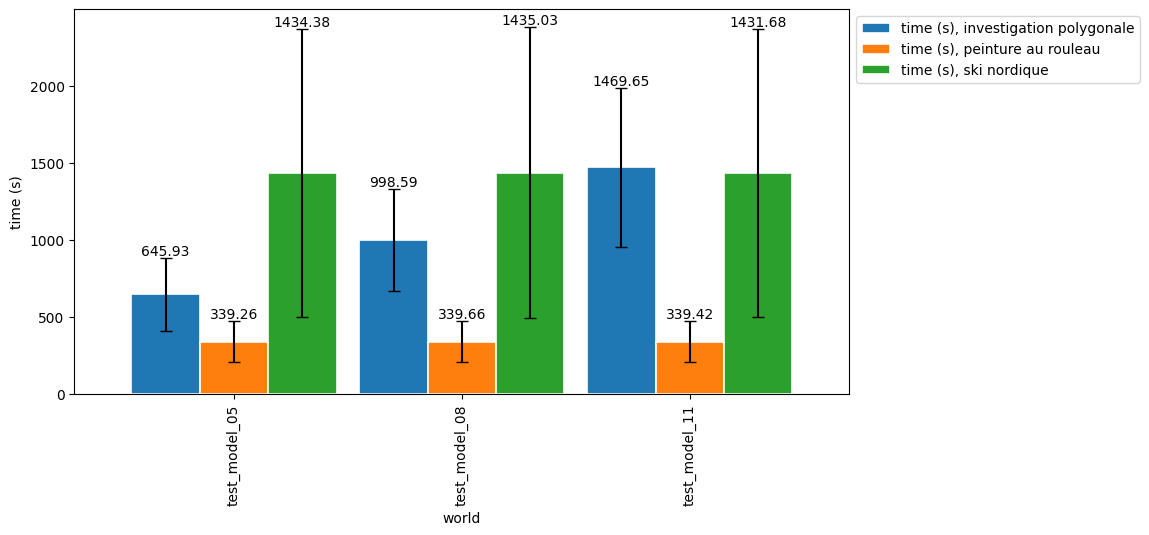
\includegraphics[width=0.49\linewidth]{graphics/investigation_polygonale-peinture_au_rouleau_ski_nordique-time_for_each_world_vs_investigation_polygonale-time_for_each_world.png}
			\end{center}

			\begin{boenumerate}\compresslist
				\item La stratégie \textit{peinture au rouleau}, a permis d'obtenir des résultats satisfaisants en des temps d'exploration très courts.
				La distance entre les robots peut être ajustée pour optimiser les résultats dépendamment de la densité des zones de corrosion inférées.
				\item La stratégie \textit{ski nordique}, a permis d'obtenir des résultats supérieurs à ceux de la stratégie \textit{peinture au rouleau}, mais avec des temps d'exploration plus longs.
				\item Enfin, la startégie \textit{investigation polygonale}, a permis d'obtenir les meilleurs résultats, en termes de précision.
				Cette stratégie réactive permet d'affiner la localisation des zones de corrosion en se basant sur les résultats d'une des deux stratégies précédentes.
				Cependant, cette stratégie est plus sensible aux collisions entre les robots, ce qui peut entraîner des résultats moins satisfaisants dans certains cas.
			\end{boenumerate}
		}
		\headerbox{6. Conclusions}{name=conclusion,column=2,below=item,span=1,above=bottom}{
			Pour la problématique d'inspection de corrosion, nous avons proposé trois stratégies de navigation multi-robots.
			Nous avons évalué ces stratégies en termes de précision et de temps d'inspection.
			Chacune de ces stratégies a montrée des résultats intéréssants.
			Les deux premières stratégies sont plus rapides, mais moins précises et permettent d'obtenir une première approximation des zones de corrosion.
			La troisième stratégie permet d'affiner la localisation des zones de corrosion en se basant sur les résultats des deux premières stratégies.

			Il serait maintenant intéréssant d'implémenter ces stratégies sur des robots réels afin de pouvoir les évaluer dans un environnement réel.
			Pour ce faire, il faudrait d'abord intégrer un système de gestion des collisions entre les robots.


		}
		% \headerbox{7. References}{name=references,column=0,span=1,below=mcs,above=bottom}{
		% 	\small % Reduce the font size in this block
		% 	\renewcommand{\section}[2]{\vskip 0.05em} % Get rid of the default "References" section title
		% 	\nocite{*} % Insert publications even if they are not cited in the poster
		% 	\bibliographystyle{unsrt}
		% 	\bibliography{rapportPFE} % Use sample.bib as the bibliography file
		% }
	\end{poster}
\end{document}